\chapter{Αποτελέσματα}
% Some examples illustrating the dependence on bunch intensity, bunch length and transverse size, plus at least on example from the multi-bunch simulations.


\section{Επίδραση παραμέτρων του επιταχυντή στην ανίχνευση της δέσμης}

\subsection{Αποτελέσματα θεωρητικού μοντέλου}
Τα αποτελέσματα της ανάλυσης που παρουσιάστηκε στην υπο-ενότητα \ref{sub:variable-analysis-MATLAB} φαίνονται παρακάτω.

\begin{figure}[tph]	
	\begin{subfigure}{0.47\textwidth}
		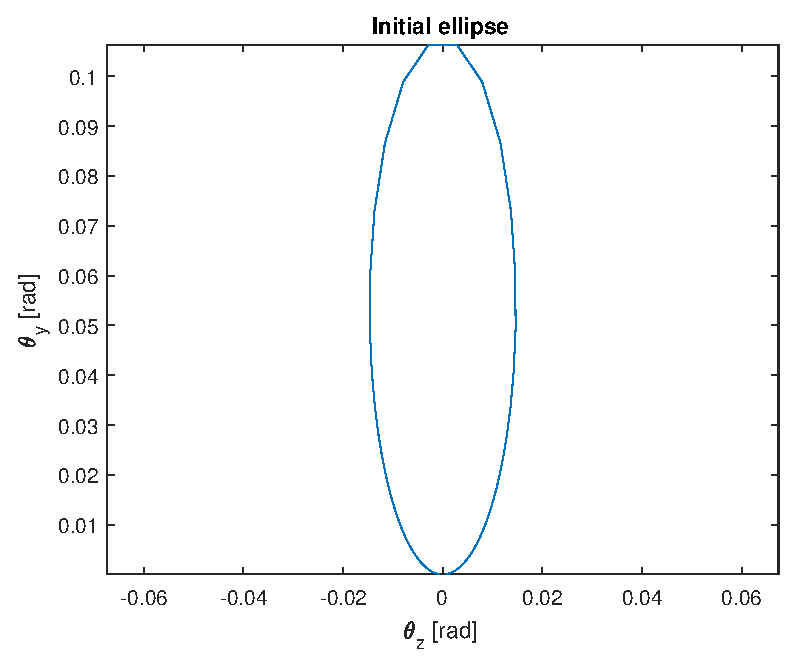
\includegraphics[width=\linewidth]{figures/MATLAB-variable-analysis/initial-ellipse}
		\centering
		\caption{Η χαρακτηριστική έλλειψη στην αρχική κατάσταση}
		\label{fig:MATLAB-variable-analysis-initial-ellipse}
	\end{subfigure}
	\hfill
	\begin{subfigure}{0.47\textwidth}
		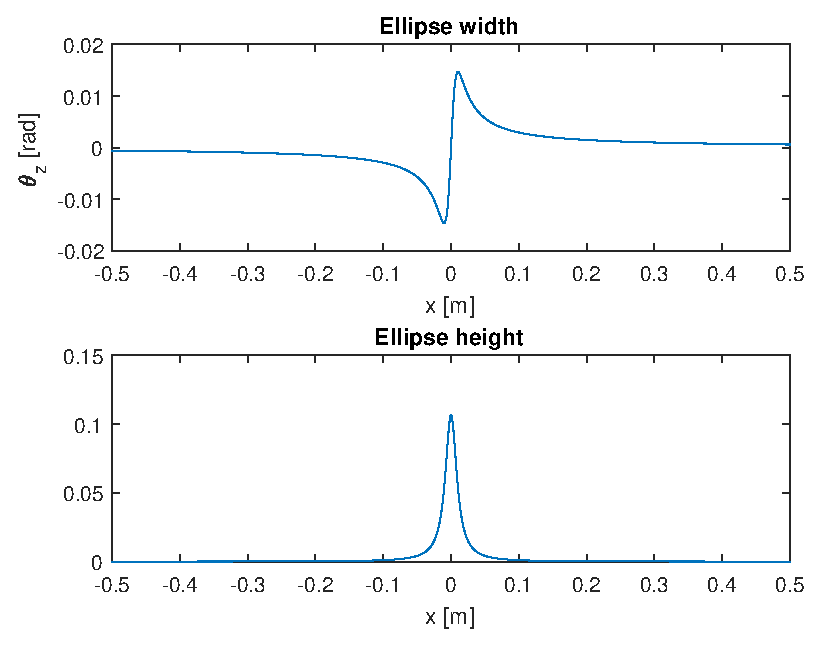
\includegraphics[width=\linewidth]{figures/MATLAB-variable-analysis/initial-ellipse-height-width}
		\centering
		\caption{Το πλάτος και ύψος της έλλειψης στην αρχική κατάσταση}
		\label{fig:MATLAB-variable-analysis-initial-ellipse-height-width}
	\end{subfigure}
\caption{Απεικόνιση και στοιχεία της χαρακτηριστικής έλλειψης στo αρχική κατάσταση}
\label{fig:initial-ellipse}
\end{figure}

\begin{figure}[tph]	
	\begin{subfigure}{0.47\textwidth}
		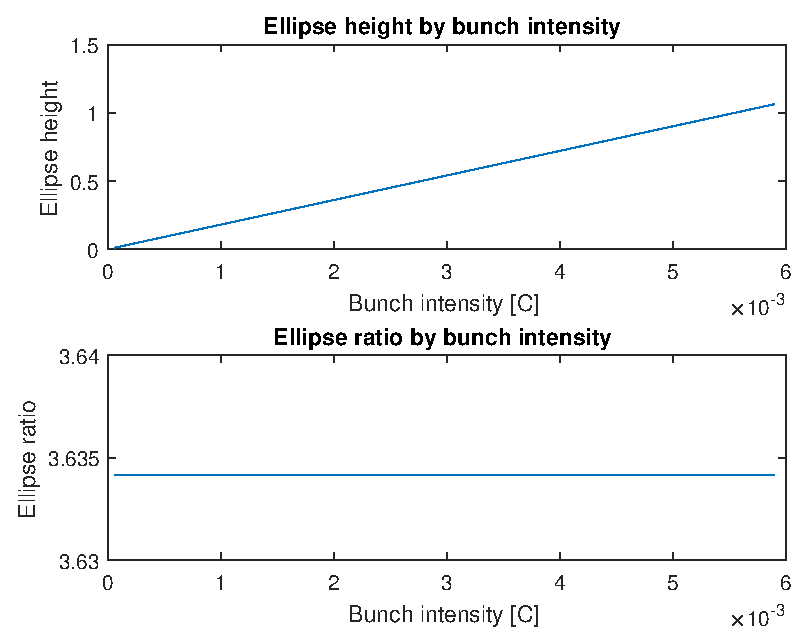
\includegraphics[width=\linewidth]{figures/MATLAB-variable-analysis/EBS-variables-intensity}
		\centering
		\caption{Επιρροή της έντασης της δέσμης ανίχνευσης στo ύψος και το λόγο της έλλειψης}
		\label{fig:EBS-variables-intensity}
	\end{subfigure}
	\hfill
	\begin{subfigure}{0.47\textwidth}
		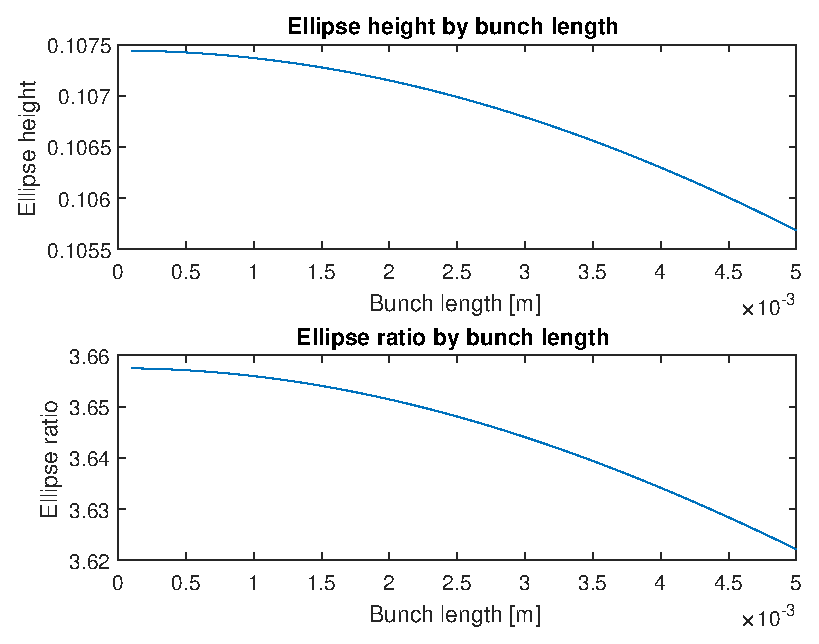
\includegraphics[width=\linewidth]{figures/MATLAB-variable-analysis/EBS-variables-length}
		\centering
		\caption{Επιρροή του μήκους της δέσμης ανίχνευσης στo ύψος και το λόγο της έλλειψης}
		\label{fig:EBS-variables-length}
	\end{subfigure}
	\par\bigskip
	\begin{subfigure}{0.47\textwidth}
		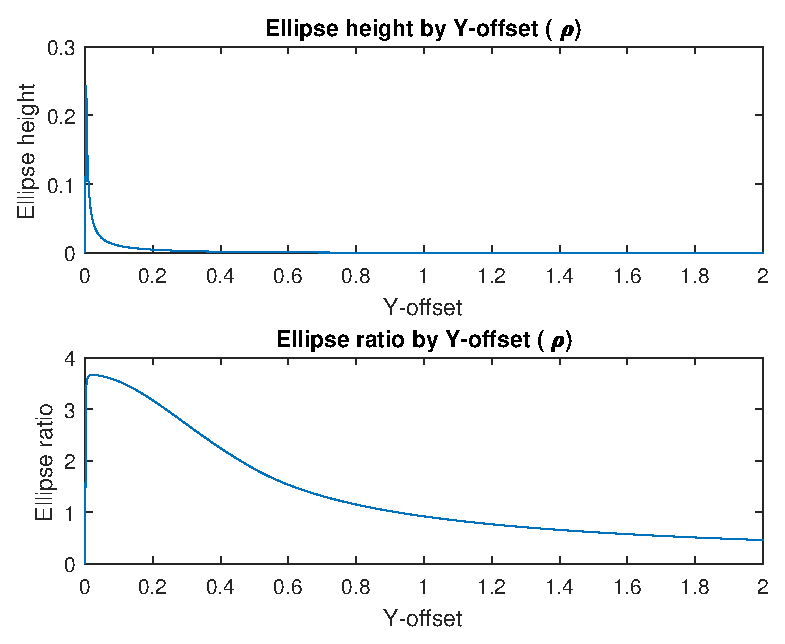
\includegraphics[width=\linewidth]{figures/MATLAB-variable-analysis/EBS-variables-rho}
		\centering
		\caption[Επιρροή της αρχικής θέσης ριπής της δέσμης ανίχνευσης στην ύψος και το λόγο της έλλειψης]{Επιρροή της αρχικής θέσης ριπής ($Y$-\en{offset}) της δέσμης ανίχνευσης στo ύψος και το λόγο της έλλειψης}
		\label{fig:EBS-variables-rho}
	\end{subfigure}
	\hfill
	\begin{subfigure}{0.47\textwidth}
		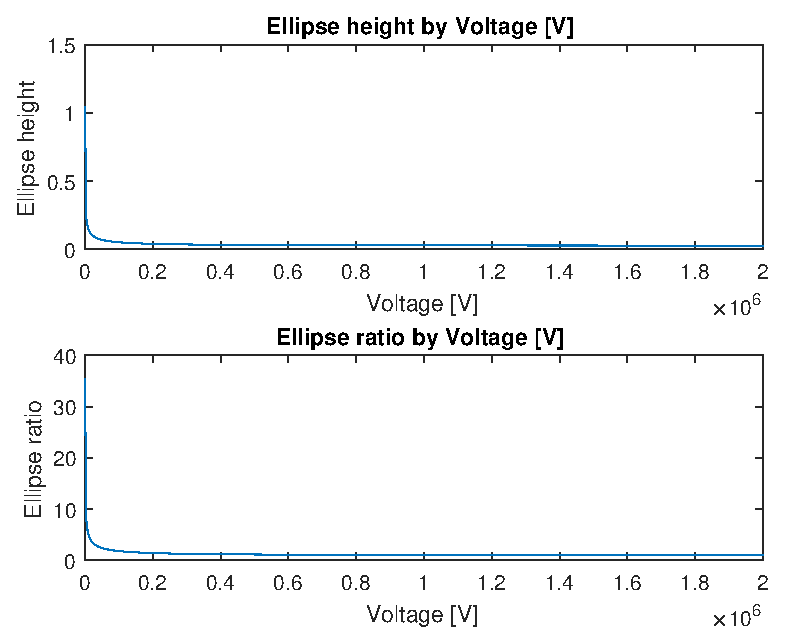
\includegraphics[width=\linewidth]{figures/MATLAB-variable-analysis/EBS-variables-voltage-linear}
		\centering
		\caption{Επιρροή της τάσης της δέσμης ανίχνευσης στo ύψος και το λόγο της έλλειψης, σε γραμμικούς άξονες}
		\label{fig:EBS-variables-voltage-linear}
	\end{subfigure}
	\par\bigskip
	\begin{subfigure}{0.47\textwidth}
		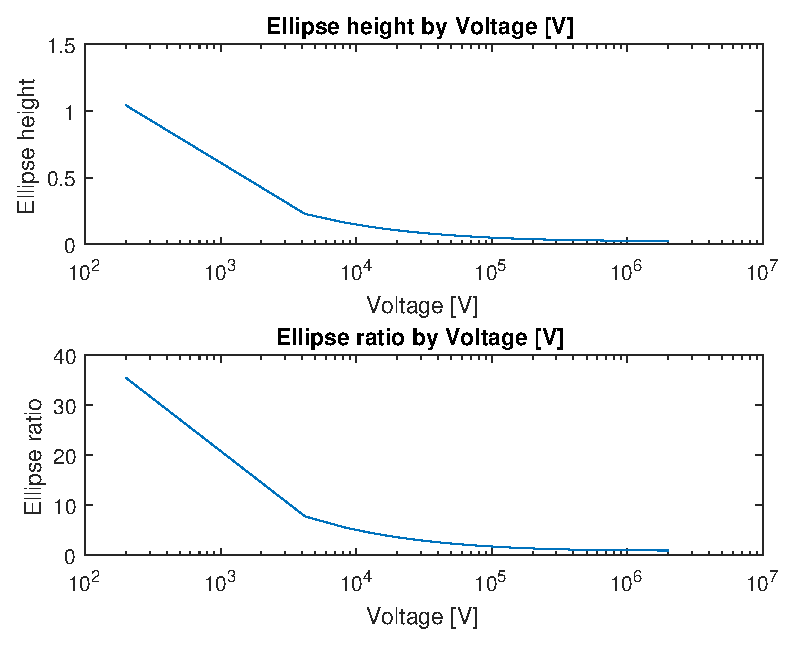
\includegraphics[width=\linewidth]{figures/MATLAB-variable-analysis/EBS-variables-voltage-log}
		\centering
		\caption{Επιρροή της τάσης της δέσμης ανίχνευσης στo ύψος και το λόγο της έλλειψης, σε ημιλογαριθμικούς άξονες}
		\label{fig:EBS-variables-voltage-log}
	\end{subfigure}
\caption{Επιρροή διαφόρων μεγεθών στη χαρακτηριστική έλλειψη}
\label{fig:beam-deflectoin}
\end{figure}

\subsection{Αποτελέσματα προσομοίωσης}
% check "Student meeting 2014-06-23" and "Student meeting 2014-08-04"



\subsection{Σύγκριση αποτελεσμάτων}

\section{Αποτελέσματα προσομοίωσης της μεθόδου στο \en{CST}}

\begin{figure}[tph]	
	\begin{subfigure}{0.8\textwidth}
		\includegraphics[width=\linewidth]{figures/CST-EBS-implementation/CST-EBS-1st-bunch-thetay}
		\centering
		\caption{Το αποτέλεσμα της προσομοίωσης για την εκτίμηση του προφίλ της 1\textsuperscript{ης} δέσμης}
		\label{fig:CST-EBS-1st-bunch-thetay}
	\end{subfigure}
	\hfill
	\begin{subfigure}{0.8\textwidth}
		\includegraphics[width=\linewidth]{figures/CST-EBS-implementation/CST-EBS-10th-bunch-thetay}
		\centering
		\caption{Το αποτέλεσμα της προσομοίωσης για την εκτίμηση του προφίλ της 10\textsuperscript{ης} δέσμης}
		\label{fig:CST-EBS-10th-bunch-thetay}
	\end{subfigure}
	\par\bigskip
	\begin{subfigure}{0.8\textwidth}
		\includegraphics[width=\linewidth]{figures/CST-EBS-implementation/CST-EBS-actual-weight-function}
		\centering
		\caption{Γραφική παράσταση της πραγματικής κατανομής της δέσμης}
		\label{fig:CST-EBS-actual-weight-function}
	\end{subfigure}
\caption{Σύγκριση της εκτίμησης για την 1\textsuperscript{η} και 10\textsuperscript{η} δέσμη, και της πραγματικής κατανομής σωματιδίων στη δέσμη στο \en{CST}}
\label{fig:CST-EBS-implementation}
\end{figure}


\section{Αποτελέσματα ανάλυσης με χρήση \en{CST} και \en{MATLAB}}




